\chapter*{Введение}\label{chap:overview}
\addcontentsline{toc}{chapter}{Введение} % This is a hack

\section{Компьютерная симуляция}

Использование компьютерного моделирования в процессе проектирования цифровых систем позволяет заметно сократить время, проходящее от момента предложения концепции новой системы до поступления на рынок первых образцов готовой продукции. Это происходит благодаря т. н. «сдвигу влево» (\textit{англ.} shift left) всей существующей методологии создания продукции, что позволяет выполнять ключевые процессы параллельно во времени, и значительноая часть из них может быть начата гораздо раньше, чем это было возможно ранее. Всё это эффективно сокращает длину цикла разработки нового продукта и увеличивает его конкурентноспособность (рис.~\ref{fig:shift-left}).

\begin{figure}[htb]
    \centering
    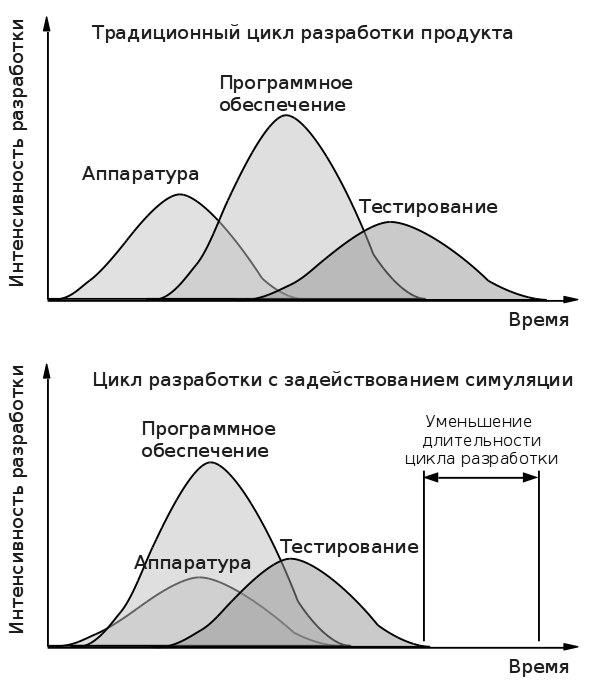
\includegraphics[width=0.7\textwidth]{./shift-left}
    \caption[Сдвиг влево]{Сдвиг влево --- возможность совместить моменты начала отдельных стадий проектирования новых цифровых систем, таким образом сокращая цикл разработки и уменьшая время вывода их на рынок}
    \label{fig:shift-left}
\end{figure}

Программное обеспечение для имитационного моделирования используется для тестирования функциональности, исследования производительности, оценки энергопотребления и иных свойств вычислительных систем на стадиях их раннего проектирования, когда реальные образцы соответствующей аппаратуры ещё недоступны. Кроме того, оно позволяет писать приложения для таких систем заранее и выпускать аппаратуру, готовую для использования конечным потребителем, не ожидая, пока все необходимые программы будут адаптированы.

Задача цикла лабораторных и практических работ, описанных в это книге, --- познакомить слушателей с новейшими достижениями в области компьютерной симуляции, связанными с эффективным созданием моделей, максимально точно представляющих аппаратные средства и при этом имеющих высокую скорость работы, получаемую благодаря эффективному задействованию имеющихся вычислительных ресурсов. Изучение проводится на программном продукте Wind River\textregistered\ Simics (в дальнейшем сокращённо называемого Simics), который в настоящее время является одним из самых современных инструментов разработки, тестирования и исследования цифровых компьютерных систем и используется как в промышленности, так и в научной среде. Несмотря на это, все рассматриваемые в книге вопросы основаны на концепциях, общих для многих других программных симуляторов, как коммерческих, так и исследовательских. В приложениях в конце книги дана информация о том, как подготовить компьютерный класс для выполнения лабораторных работ на Simics.

Для максимально эффективного усвоения материала данного пособия читателю рекомендуется иметь начальные знания по архитектуре ЭВМ. Желательно иметь понимание общих принципов работы операционных систем, а также знакомство с языками программирования высокого уровня и ассемблера. Базовой операционной системой для запуска приложений в практических работах служит GNU/Linux; для более чёткого понимания используемых в работах операций читатель должен быть знаком с работой интерпретатора командной строки Unix.

\section{Обозначения}
При первом использовании в тексте терминов, заимствованных из английского языка и не имеющих известных авторам общепринятых переводов на русский язык, в скобках после них будут указываться оригинальные выражения.

Всюду в тексте данной работы будут использованы следующие шрифтовые выделения и обозначения.

\begin{itemize*}
    \item Обычный текст используется для основного материала.
    \item \texttt{Моноширинный текст} вводится для исходных текстов программ на различных (псевдо) языках программирования и их ключевых слов,  имён регистров устройств, листингов машинного кода, результатов работы операторов командной строки.
    \item \textit{Курсивный текст} используется для выделения новых понятий.
    \item \textbf{Полужирный текст} используется для обозначения элементов графического интерфейса: имён окон, пунктов меню и т.п.
    \item Числа в шестнадцатеричной системе счисления имеют префикс \textbf{0x} (например, 0x12345abcd), в двоичной системе счисления --- суффикс \textbf{b} (например, 10010011b).
    \item Команды, которые необходимо вводить в строку приглашения запущенного Simics, имеют префикс \texttt{simics>}:
    \begin{lstlisting}
simics> list-objects
    \end{lstlisting}
	Ответный вывод команд, если он есть, приводится без каких-либо предваряющих префиксов. Если вывод очень длинен, то часть его заменяется многоточием.
    \item Команды, которые необходимо вводить в строку приглашения интерпретатора (в данной книге используется стандартный \texttt{/bin/sh}), имеют префикс \texttt{\$} для обычного пользователя или \texttt{\#} для команд, выполняемых суперпользователем root:
    \begin{lstlisting}
$ ./simics targets/x86-x58-ich10/viper.simics
# mount /dev/sdb /mnt/disk
    \end{lstlisting}

    \item При описании синтаксиса команд их обязательные аргументы команд указываются в угловых скобках, необязательные --- в квадратных:
    \begin{lstlisting}
$ command <mandatory argument> [optional argument]
    \end{lstlisting}
	Если команда принимает несколько однотипных аргументов подряд, спользуется многоточие \texttt{...} для второго и последующих параметров.
\end{itemize*}

